\documentclass{article}
\usepackage{tikz}
\usetikzlibrary{matrix, calc, positioning, arrows}
\usepackage{fontspec}
\setmainfont{[EncodeSans-Regular.ttf]}
\newfontfamily{\bold}{EncodeSans-Bold.ttf}
\usepackage{xcolor}
\definecolor{capri}{RGB}{0, 153, 215}
\begin{document}

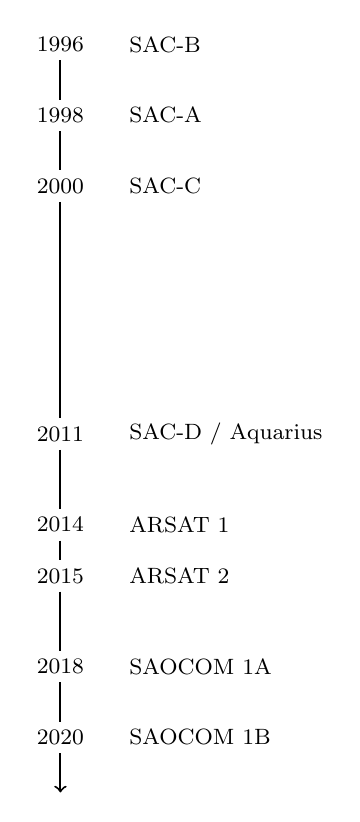
\begin{tikzpicture}

% 1 -> 0.25
% 2 -> 0.5
% 3 -> 0.75
% 11 -> 2.75

\draw[line width=0.25mm, -] (0,20) -- (0,19.5);
\draw[line width=0.25mm, -] (0,19.1) -- (0,18.6);
\draw[line width=0.25mm, -] (0,18.2) -- (0,15.45);
\draw[line width=0.25mm, -] (0,15.05) -- (0,14.30);
\draw[line width=0.25mm, -] (0,13.9) -- (0,13.65);
\draw[line width=0.25mm, -] (0,13.25) -- (0,12.5);
\draw[line width=0.25mm, -] (0,12.1) -- (0,11.6);
\draw[line width=0.25mm, ->] (0,11.2) -- (0,10.7);

% Add the years as labels
\node at (0, 20.2) {\footnotesize \bold{1996}};
\node [right] at (0.75, 20.2) {\footnotesize SAC-B};

\node at (0, 19.3) {\footnotesize \bold{1998}};
\node [right] at (0.75, 19.3) {\footnotesize SAC-A};

\node at (0, 18.4) {\footnotesize \bold{2000}};
\node [right] at (0.75, 18.4) {\footnotesize SAC-C};

\node at (0, 15.25) {\footnotesize \bold{2011}};
\node [right] at (0.75, 15.25) {\footnotesize SAC-D / Aquarius};

\node at (0, 14.1) {\footnotesize \bold{2014}};
\node [right, align = left] at (0.75, 14.1) {\footnotesize ARSAT 1};

\node at (0, 13.45) {\footnotesize \bold{2015}};
\node [right] at (0.75, 13.45) {\footnotesize ARSAT 2};

\node at (0, 12.3) {\footnotesize \bold{2018}};
\node [right] at (0.75, 12.3) {\footnotesize SAOCOM 1A};

\node at (0, 11.4) {\footnotesize \bold{2020}};
\node [right] at (0.75, 11.4) {\footnotesize SAOCOM 1B};

\end{tikzpicture}

\end{document}